\documentclass[11pt]{article}

\usepackage{graphicx} % Required for inserting images
\usepackage[letterpaper, margin=1in]{geometry}
\usepackage{parskip}

\usepackage{amsmath}

\title{The Propagation of Political Beliefs in Social Networks}
\author{Daniel Popp \and Marcelo Beramendi Caballero}
\date{April 19th, 2023}

\begin{document}

\maketitle

\section{Explanation and Motivation}

\subsection{Propagation of Political Beliefs}

The political ideology of individuals can be understood as the collection of their beliefs across a variety of subjects. A common way of representing political ideology is with a political spectrum, where political topics are grouped depending on their nature. One of the most common ones is the left-right division, which refers to the economic beliefs of people. 

Left wing economics tends to favor State intervention to protect worker rights, high tariffs on imports to protect local industries, state-owned social services, and similar policies. On the other hand, right wing economics favor the free market, low taxes for foreign investors who want to do business in the country, privatization of social services, and other similar policies.

It is possible for an individual to have a left-leaning stance on some topics, and a right-leaning stance on others. For example, several Republican politicians, including Donald Trump, support lower taxes for high-income people, but also support protectionist economic measures which are often associated with the left. Therefore, it is best to understand political beliefs as distributions, instead of as entirely left or right-leaning.

Different populations often end up with different average political beliefs. For example, the U.S. has historically favored free markets and economic liberty much more than Nordic countries like Denmark and Norway, where social democrat and labour parties are very popular. However, even within one population, there are often ideological shifts in the beliefs of individuals.

In this paper, we want to study the factors that drive ideological change in social networks. We will study how populations with different beliefs interact with each other, and how external influences can shift the ideology of populations. We will approach this problem using an agent-based modeling approach.


\subsection{Agent-Based Models of Social Dynamics}

Complex social dynamics can emerge from the individual characteristics of people's cognitive processes. Just like bird flocking emerges from very simple rules of how individual birds behave \cite{christodoulidi2015phase}, political and sociological events can also be studied by looking at the individual cognitive and emotional characteristics of the people who participate in society. For example, in \textit{The Righteous Mind}, Jonathan Haidt argues that people are mainly guided by intuition, and not by rationale \cite{haidt2012righteous}. He explains that the reason people from political opposites often don’t listen to each other is that humans often reach conclusions first, and then think of reasons to justify their conclusions, which can be seen when analyzing people’s brain activation patterns \cite{saletan2012why}. This is very relevant, because it is an explanation of political polarization, a large political phenomenon, from the very basic, individual rules that guide people’s thought processes.

Another great example of how social dynamics emerge from simple cognitive processes is mentioned by David Livingstone Smith in his book \textit{Less Than Human}. Smith looks at the psychological and physiological characteristics of people to study the phenomenon of dehumanization. He argues that dehumanization is a psychological defense mechanism ingrained in human cognition that allows people to mistreat and exploit others, and analyzes how language, imagery and ideology are often used to dehumanize groups of people. He believes that dehumanization, a phenomenon that starts as an individual cognitive phenomenon, is what leads to large scale atrocities like genocides and slavery \cite{smith2011less}. 

Approaching complex dynamics from the behavior of individual agents is also a common technique when building computational models. Computational models are often used to study political and sociological phenomena \cite{cederman2005computational, kim2020computational, scott2003computational}. Several researchers have approached computational modeling of politics and sociology by using agent-based models, where the interactions between agents produce large-scale behaviors \cite{bianchi2015agent, bruch2015agent}.

Approaching these types of problems with an agent-based modeling approach is very beneficial, because it allows for the formulation of much more specific hypotheses. Qualitative models are inherently limited, because while they may be able to make general, broad predictions of what will happen in the future, they are not capable of predicting how quantitative changes in the characteristics of populations will affect the overall dynamics of the system. Therefore, it is very appealing to take qualitative models of social dynamics, and use them to build computational models that are able to make both qualitative and quantitative predictions. This allows to, for example, study how the quantitative variation of parameters that are used to represent real-world characteristics affects the dynamics of the system. This background provides the motivation for creating an agent-based model of political belief propagation.

Since we are creating an exploratory simulation of human behavior, rather than a data-driven model, success is a qualitative measure. Our goal is to create a feasible model of the propagation of political beliefs, so if the results of our simulations match the intuition about the social dynamics which could be used to interpret a given network, we consider that a success.

\section{Approach}

We developed an agent-based model of the propagation of political beliefs within social networks. We model political beliefs of an individual agent by a beta distribution. Beliefs are propagated through conversations where ``evidence" is sampled based on the conversation partner's beliefs. These conversations serve as the connections between agents in a larger social network, in which we can monitor the spread of beliefs over time.

\subsection{Modeling Political Beliefs}

We model political beliefs with a beta distribution. This is a probability distribution with density function \[p(x|\alpha, \beta) = \frac{1}{B(\alpha, \beta)}x^{\alpha-1}(1-x)^{\beta-1},\] where \(B(\alpha,\beta)\) is a normalizing constant defined with the Gamma function as \(\frac{\Gamma(\alpha)\Gamma(\beta)}{\Gamma(\alpha+\beta)}.\)

The distribution could be interpreted as an answer to the question “What proportion of economic policy should be right wing?” Each person then has a beta distribution representing their beliefs about this proportion, where someone who is “left-wing” would have a denser distribution to the left of 0.5, and a “right-wing” person would have a denser distribution to the right of 0.5. This is extremely oversimplified compared to the complexities of true political belief, but it is sufficient to develop an interesting simulation. While it simplifies political beliefs to probabilities regarding a single variable, the beta function is flexible in shape, allowing for the distinction of various ideological beliefs.

\begin{figure}[h]
\centering
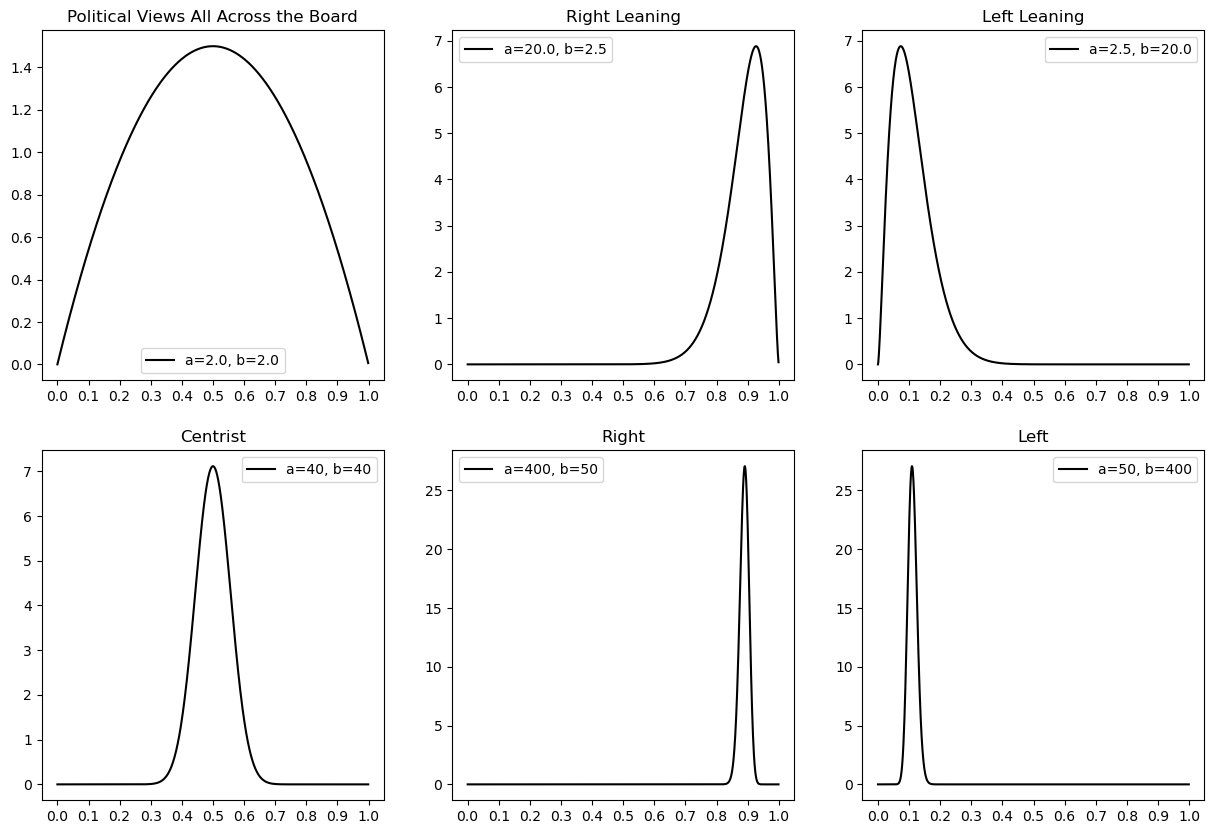
\includegraphics[scale=0.5]{images/modeling_beliefs.png}
\caption{Various parameterizations of the beta distribution representing types of political beliefs.}
\end{figure}

\subsection{Updating Beliefs}

Bayes' theorem provides a probabilistic tool to model how beliefs update when given more evidence. 

The beta distribution is considered the \textit{conjugate prior} of the Bernoulli distribution because multiplying a beta distribution times a Bernoulli distribution grants another beta distribution. This means that, rather than multiplying distributions to get the posterior belief distribution, we can derive rules to update the parameters to the beta distribution based on the evidence sampled from the Bernoulli distribution, granting a less computationally expensive way of updating beliefs.

In the case of a beta prior, $\text{Beta}(\alpha, \beta)$, with evidence sampled from a Bernoulli likelihood, $\text{Ber}(\theta)$, described by the sample size, $n$, and the number of samples which yielded 1, $y$, the posterior distribution is $\text{Beta}(\alpha*,\beta*)$, where 
\begin{align*}
\alpha* &= \alpha + y \\
\beta* &= \beta + n - y
\end{align*}

Human beings, however, are not perfectly rational. When provided evidence, our beliefs do not really update following Bayes' theorem. To model this, we add two extra parameters to the update rules:
\begin{align*}
\alpha* &= \alpha + OM \cdot T \cdot y \\
\beta* &= \beta + OM \cdot T \cdot (n - y)
\end{align*}

$OM$ represents the agent's ``open-mindedness." An agent with a perfect open-mindedness coefficient would update beliefs similarly to the ``rational" update rules derived from Bayes' theorem. While the parameter can have any value, we will primarily use $0 < OM < 1$ to model confirmation bias, where people are more likely to interpret evidence as supporting their current beliefs. This means the beliefs will update slower in the face of evidence than would be considered rational by Bayes' theorem.

The other parameter, $T$, represents trust. This comes into play when we model the propagation of beliefs through a social network, since the evidence used to update beliefs is being sampled from other agents, not some ``ground truth" distribution. Humans will trust different sources to various degrees, so we will respond faster to agree with people we trust faster than people we do not. Even an open minded individual can be reluctant to update their beliefs if they are speaking to someone who they trust very little.

Together, these parameters control how an agent's beliefs are updating from a given conversation.

However, one limitation of using beta distributions is that the more beliefs update, the narrower the distribution becomes. This is because after observing a larger amount of evidence, beliefs start becoming more defined. However, this is not representative of how political beliefs work. An individual could potentially shift their beliefs towards one side, without narrowing down their beta distribution. This would happen if you receive a lot of conflicting evidence for very few talking points, because while the amount of evidence would increase by a lot, your answer to the question  “What proportion of economic policy should be right wing?” would not narrow-down too much, because the evidence only belonged to very few points.

To represent this, we further modified the way beliefs are updated such that the values of alpha and beta change, but the total amount of evidence (alpha + beta) is a little resistant to changes. With this update, it is still possible to shift someone's beliefs, but it takes a little more effort to change how narrow the beta distribution of an agent is. After updating parameters, they are ``recalibrated" so that the sum of the parameters stays similar. This is done by first calculating the desired sum of the parameters, $n_{new}$,
\begin{align*}
    n_{self} &= \alpha* + \beta*\\
    n_{other} &= \alpha_{other} + \beta_{other}\\
    n_{new} &= 0.95 \cdot n_{self} + 0.05 \cdot n_{other}.
\end{align*}

$\alpha*$ and $\beta*$ are then each scaled using this new value to recalibrate their sum:
\begin{align*}
    \alpha*_{calibrated} &= \alpha* \cdot \frac{n_{new}}{n_{self}} \\
    \beta*_{calibrated} &= \beta* \cdot \frac{n_{new}}{n_{self}}.
\end{align*}


\subsection{Modeling Conversations}

Rather than observing evidence from a ground truth distribution, we simulate conversations by sampling from the other person's distribution. This would represent the different political conversation points that are brought up during a conversation. To do this, we generate a sample from the other person's beta distribution. These values are then used as the parameters to Bernoulli distributions. A data point is sampled from each of these Bernoulli distributions, at which point we can easily calculate $y$ and $n$ and update the beliefs according to the rules described above. This makes sense because if the beta distribution of an individual is, for example, more left-leaning, then it is more likely that they will mention left-leaning stances when talking about politics.

Below is an example of beliefs update after a conversation.

\begin{figure}[h]
\centering
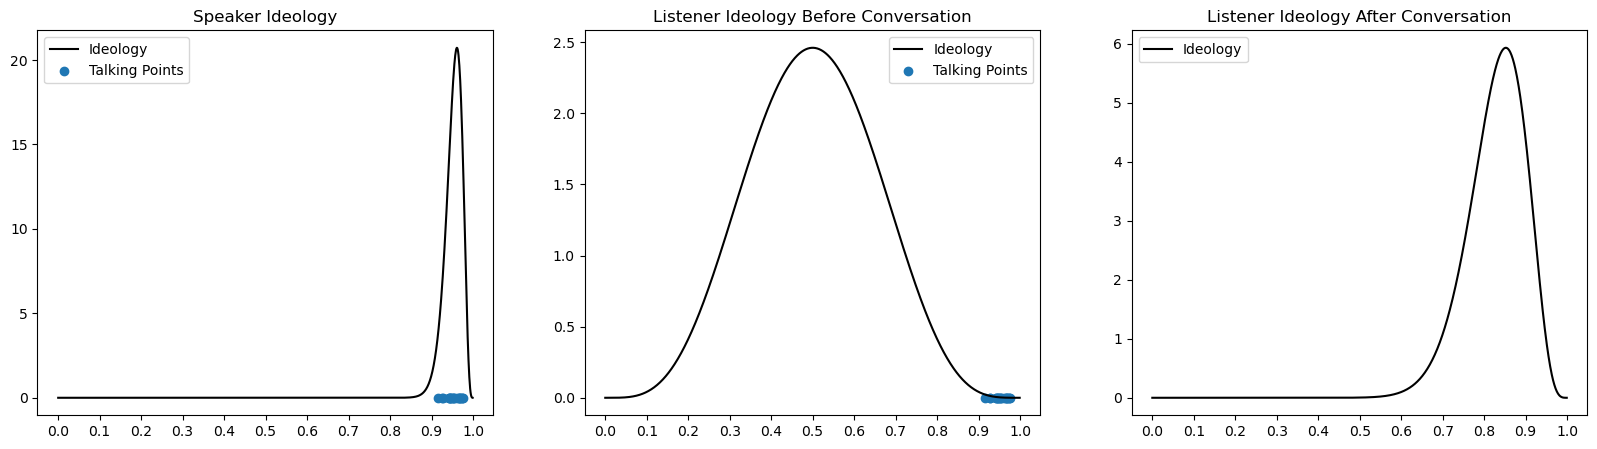
\includegraphics[scale=0.4]{images/modeling_conversation.png}
\caption{An example of a conversation with one speaker and one listener. The beliefs of the listener are updated after listening to the speaker.}
\end{figure}

% \newpage

\subsection{Modeling Social Networks}

We then combine everything together to whole social networks. The nodes of these networks are individual people, whose political beliefs are represented by a beta distribution, and who each have an open-mindedness parameter, typically in the range $0<OM<1$. The edges of the network represent correspondences. Edges are directed, with a source person sending information to a target person, with which the target person's beliefs are updated.

Edges have a few additional parameters associated with them. First is trust, which is used in the update equations for beliefs. The next parameter is frequency, which represents how often this correspondence happens. The network is updated with time steps representing one day, and the frequency represents the probability that the correspondence happens on a given day. The final parameter is magnitude, which represents how the size of the sample sent as ``evidence," which could be interpreted as the length of the conversation or how much information is transmitted in the conversation.

\section{Results}

\subsection{Demonstration of Parameter Effects}

We will start by briefly demonstrating the effects of the open-mindedness and trust parameters. In all examples in this subsection, the frequency and magnitude of each relationship are set to 1 and 10, respectively. We will not demonstrate frequency and magnitude individually to save space, as their effects are pretty intuitive, and serve more to add more depth to the types of relationships which can be represented in larger social networks. For example, a person could trust very closely a significant other and a childhood friend, but they would talk to their significant other far more often.

\subsubsection{Open-Mindedness}

We start with a simple model with two people. One person is the "Listener," who's open-mindedness we will vary, and the other person is the "Speaker." The evolution of the Listener's beliefs is demonstrated in the plot below.

\begin{figure}[h]
    \centering
    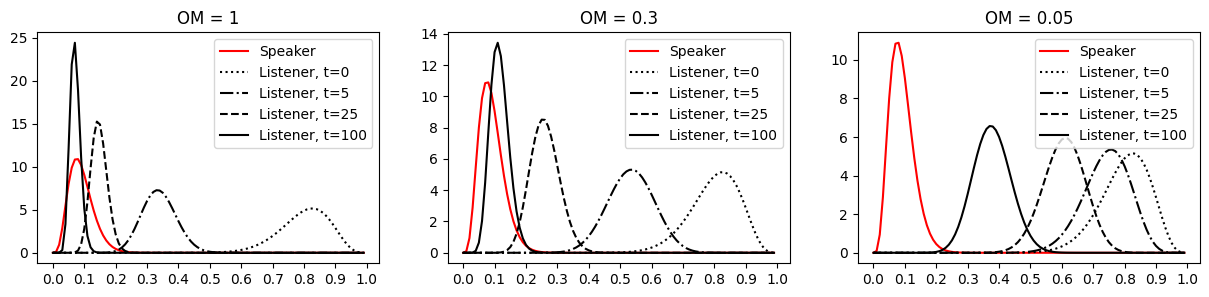
\includegraphics[scale=0.5]{images/open_mindedness_example.png}
    \caption{The evolution of beliefs with listeners of varying open-mindedness.}
\end{figure}

This result demonstrates an intuitive reflection of human behavior. The more open-minded the individual, the faster their beliefs converge to the evidence provided by their conversation partner. A less open-minded individual will still update their beliefs, but are more skeptical and require more evidence.

\subsubsection{Trust}

When there is only one source of information, trust acts in the same way as open-mindedness. As demonstrated in the plot below, when trust is low, it takes longer for beliefs to converge.

\begin{figure}[h]
    \centering
    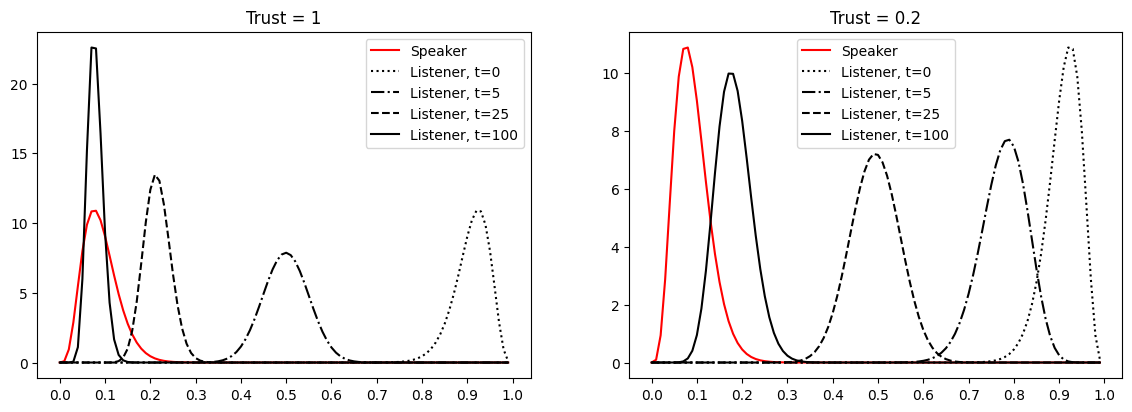
\includegraphics[scale=0.5]{images/trust_example.png}
    \caption{The effect of trust in a simple one-way conversation. When trust is lower, beliefs take longer to shift.}
\end{figure}

\newpage

Trust becomes interesting when there are multiple sources of information. In this next example, there is one person who is talking to two people with opposite views. When the listener trusts both sources equally, their beliefs stay somewhere in the middle. However, if the listener trusts one source more than the other, their beliefs will shift over time.

\begin{figure}[h]
    \centering
    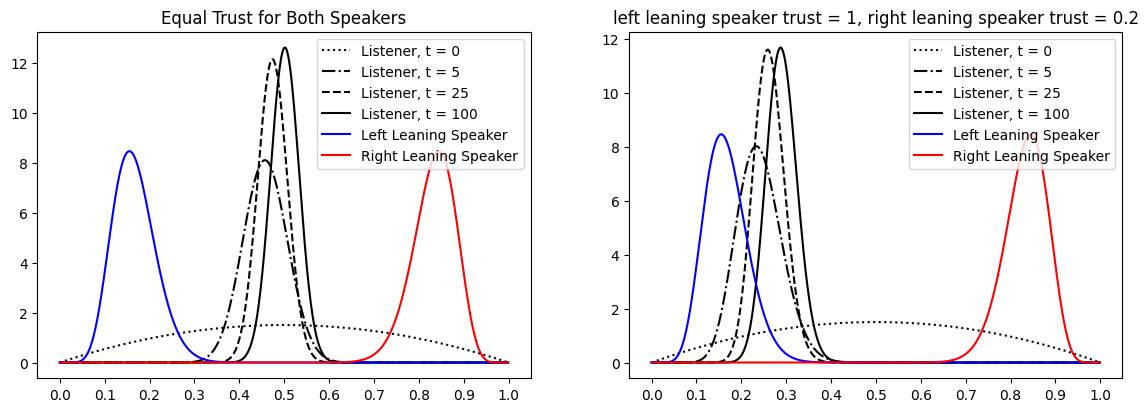
\includegraphics[scale=0.5]{images/trust_two_sources.png}
    \caption{The effect of trust in a network with more people. When a person is receiving equal amounts of information from two opposing people, their beliefs shift in the direction of the person they trust more.}
\end{figure}

\newpage

\subsubsection{Combined Effects}

By varying the open-mindedness of the listener in the previous two-speaker example, we can see the combined effects of open-mindedness and trust. As before, when trust is equal, beliefs stay in the middle, but condense faster when open-mindedness is higher. When trust is unequal, beliefs shift to the side of higher trust, but faster and more compacted when open-mindedness is higher.

\begin{figure}[h]
    \centering
    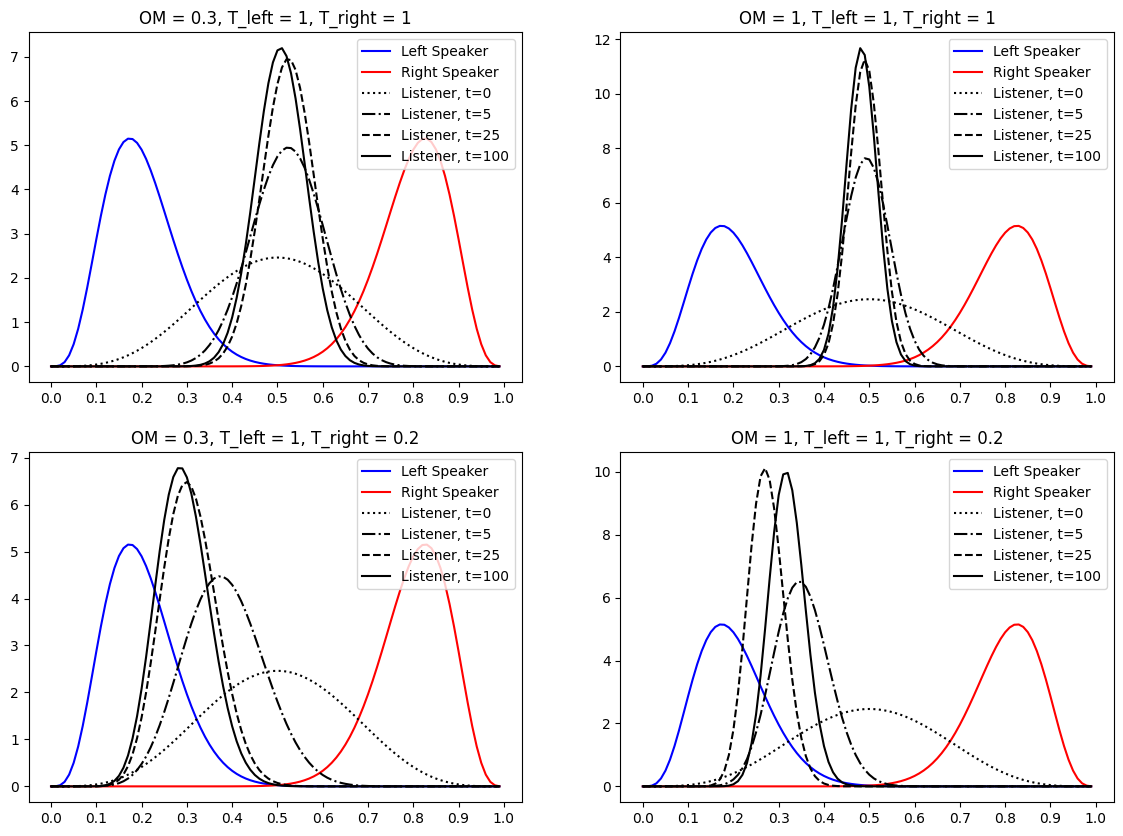
\includegraphics[scale=0.5]{images/trust_and_OM_example.png}
    \caption{Plots demonstrating the combined effects of trust and open-mindedness in a simple 3-person network.}
\end{figure}

\subsection{Larger Networks}

Now that we have seen how individuals can update their beliefs when interacting with others, we will use that design to study large-scale social dynamics. To do this, we will large networks of people and shape their structure to represent real situations. The goal of this is to test whether real-world social dynamics are capable of emerging from the modeled rules of how individuals update their beliefs.

\subsubsection{Two social groups connected through one person}

Consider the following network, where two distinct social groups are connected by one individual. This could represent a scenario such as a college student being a link between their college and their hometown.

In this example, one of the social groups has left-leaning political beliefs, and the other has right-leaning political beliefs. The trust, frequency, and magnitude parameters were randomly generated for each individual. However, the sampling distributions were designed so that people within a group talk more often and typically have a higher trust, within the range $(0.8,2)$, whereas the connections with the center person are slightly less frequent and have moderate trust, within the range $(0.7, 1.3).$ The important idea to keep in mind is that the center person frequents and trusts both groups in similar levels. The generated social network is depicted below.

\begin{figure}[h]
    \centering
    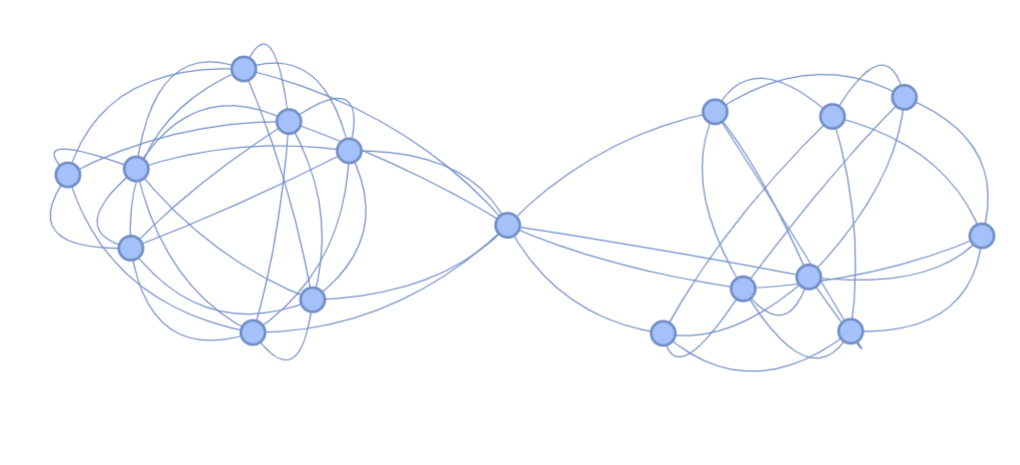
\includegraphics[scale=0.8]{images/two_social_groups_network.png}
    \caption{A social network where two distinct groups with opposing beliefs are connected by a single person.}
\end{figure}

This network was simulated for 100 time steps. The evolution of beliefs of the intermediary person, and a random person from each of the two social groups is depicted below.

\begin{figure}[h]
    \centering
    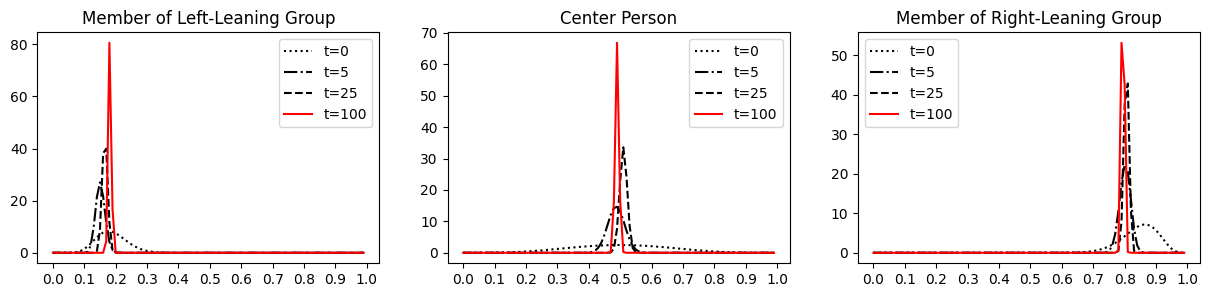
\includegraphics[scale=0.53]{images/two_social_groups_individual_beliefs.png}
    \caption{The evolution of beliefs of three individuals from the network}
\end{figure}

Unsurprisingly, the center person's beliefs stay in the middle because they are receiving conflicting information from each of their social groups at approximately symmetric frequencies and magnitudes with approximately symmetric trust. The members of the right and left groups tend slightly towards the middle, since each group the center person is slightly pulling each group in. To demonstrate this farther, we also plot the evolution of the average beliefs of each social group.

\begin{figure}[h]
    \centering
    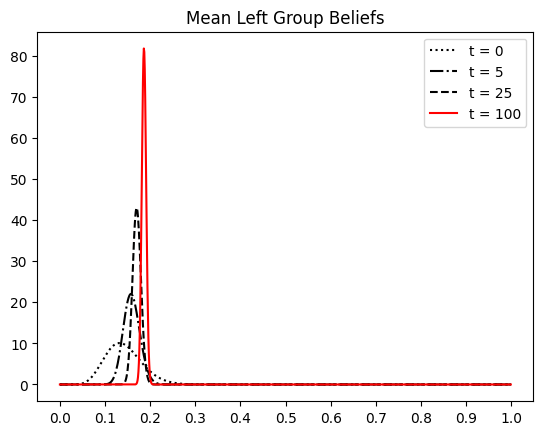
\includegraphics[scale=0.4]{images/two_social_groups_mean_left.png}
    \hspace{1cm}
    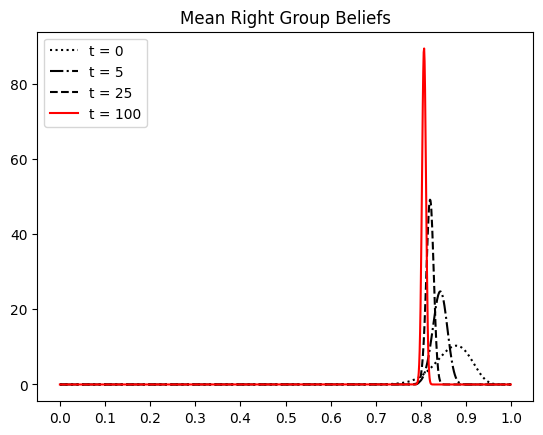
\includegraphics[scale=0.4]{images/two_social_groups_mean_right.png}
    \caption{The evolution of the average beliefs within each of the distinct social groups.}
\end{figure}

\newpage

We will now slightly modify this example to model the college student example slightly better. The center person will start with beliefs similar to one group, but talk to that group less since they are no longer home. Their new social group at college has opposing political beliefs, but they talk much more often.

\begin{figure}[h]
    \centering
    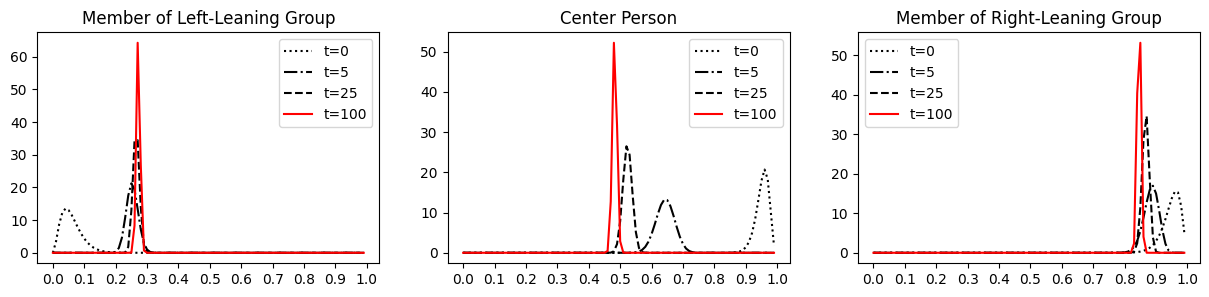
\includegraphics[scale=0.5]{images/two_social_groups_diff_freq_individual_beliefs.png}
    \caption{The evolution of beliefs of three individuals from the network: one person from the right-leaning "home" social group, one person from the left-leaning "college" social group, and the college student who transitioned social groups.}
\end{figure}

We can see that the dynamics are different this time. The college student starts with right-wing beliefs, but after moving to a left-wing social group, their beliefs are pulled to the left. Perhaps more interesting here is the difference in the shift in beliefs between members of each of the social groups. We can see that with the introduction of a right-wing member to the largely left-wing social group, the beliefs of a member of are pulled more to the center than the beliefs of the right-wing home social group are moved. This makes sense, because the college social group is influenced by someone with completely different beliefs, whereas for most of the simulation, the home group is still communicating with someone who leans right, just less so than they used to. These dynamics are again demonstrated better by the average beliefs of each social group.

\begin{figure}[h]
    \centering
    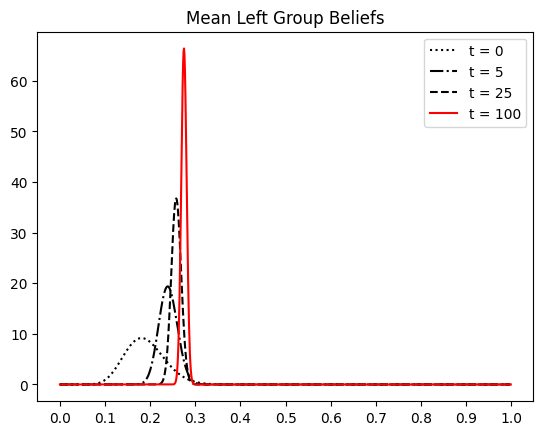
\includegraphics[scale=0.4]{images/two_social_groups_diff_freq_left_mean.png}
    \hspace{1cm}
    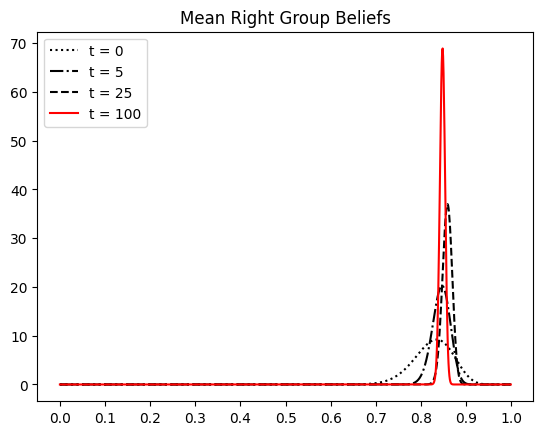
\includegraphics[scale=0.4]{images/two_social_groups_diff_freq_right_mean.png}
    \caption{The evolution of the mean beliefs of the old and new social groups.}
\end{figure}

\subsubsection{Modeling the effect of news media in the political ideology of the population}

The political ideology of populations is not isolated from external influence. There are several sources that push the beliefs of populations in different directions, such as politicians and social media. However, when it comes to influencing the beliefs of populations, one of the most powerful sources are news media. We will model the effect that news media has on populations.

In this example, agents in the population have randomly generated starting ideologies with both alpha and beta parameters starting within range (60,160). On average, the starting beliefs of the population will lean towards the center, but each agent will have different starting points. The amount of connections, trust, frequency and magnitude of conversation of agents was also randomly generated. 

In addition, we added two different nodes to represent news media. One of them has political beliefs towards the far-right, and the other towards the center-right.  News media reach much more people than the average individual, so we gave them significantly more connections. In addition, while news media can transmit their ideas to people, people do not shape the ideology of news media companies. It is also the case that different individuals can trust different news sources to different degrees. Trust values were set to represent this.

The image below shows the generated population of 50 people in blue, and both news media sources in red.

\begin{figure}[h]
    \centering
    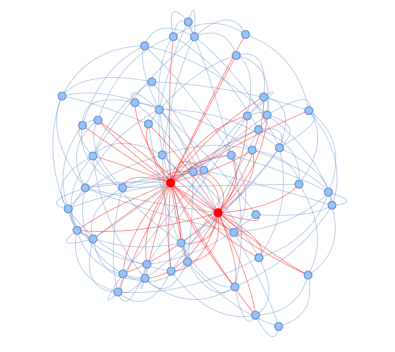
\includegraphics[scale=0.7]{images/News media simulation.png}
    % \hspace{1cm}
    \caption{A social network where there are two news media sources. One media source is to the far-right, and the other is to the center-right.}
\end{figure}

This network was simulated for 100 time steps. The evolution of beliefs of two random people in the population are shown in the image below.

\begin{figure}[h]
    \centering
    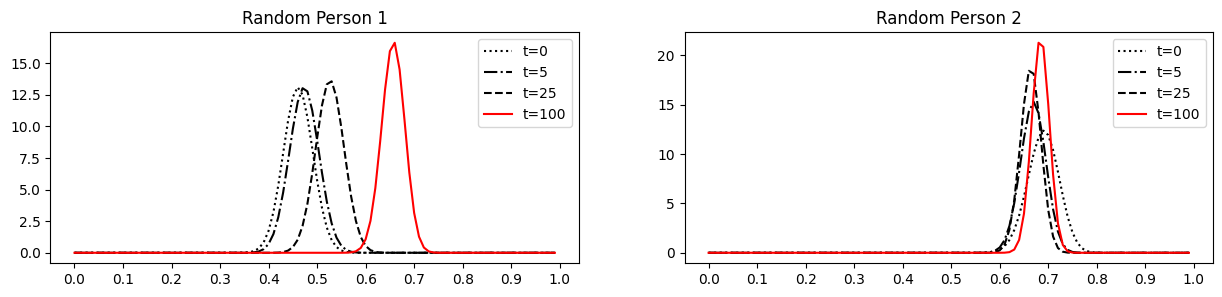
\includegraphics[scale=0.5]{images/Random people from news media simulation.png}
    % \hspace{1cm}
    \caption{The evolution of the beliefs of two random people from the network.}
\end{figure}

We can see that Random Person 1 starts with political beliefs aligned to the center, but as they spend more time in the network, news media sources push their beliefs towards the right. We can also see that Random Person 2 already starts with beliefs that alight with the center-right, so their beliefs do not change much with time. These results show that individuals in the network are behaving as expected, which points towards the fact that our modeled agents are capable of representing real-world behaviors.

We can also see how the mean beliefs of the population change under the influence of social media in the figure below.

\begin{figure}[h]
    \centering
    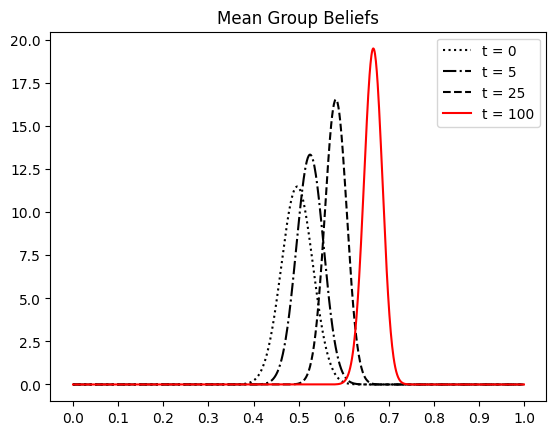
\includegraphics[scale=0.6]{images/Mean group beliefs from news media simulation.png}
    % \hspace{1cm}
    \caption{The evolution of the beliefs of two random people from the network.}
\end{figure}

The beliefs of the population behave as expected. If there are only news media sources pushing towards one side of the political spectrum, then it is natural that the ideology of the population shifts towards that side. This results are great, because they show that our model is capable of representing the social dynamics of news media.

\subsubsection{Modeling the effect of radical ideologies in the population. How do echo chambers affect the propagation of political beliefs?}

What happens when a couple individuals in the population become radicalized towards one side of the political spectrum? Historically, groups with extremist beliefs have always emerged, and in many cases they have lead to wars and genocides. The propagation of extremist beliefs usually happens through the formation of echo chambers, where people of similar radical ideologies influence each other, so they end up resisting changing their beliefs.

We test our model's ability to represent extremist beliefs by generating a large network of 60 people with similar characteristics as in the previous example. However, 8 of those 60 people are defined to be right-wing extremists, with alpha = 400 and beta  = 50.

We want to test how the structure of the network affects the propagation of beliefs, so we will have two different networks. In the first network, extremists will be randomly spread across the population. In the second network, extremists will form small groups of 2 to 3 people. Amongst these groups, they will frequent and trust each other more than other people in the network. In Network 2, right-wing extremists will be more likely to approach other people to talk to them, since once extremists find each other they usually start wanting to spread their beliefs. 

Note that in both of these networks, in contrast with the news media network, the beliefs of extremists are subject to the influence of the rest of the population. We will see how the political ideology of both the non-extremist and  extremist populations evolve with time. The image below shows both networks.

\begin{figure}[h]
    \centering
    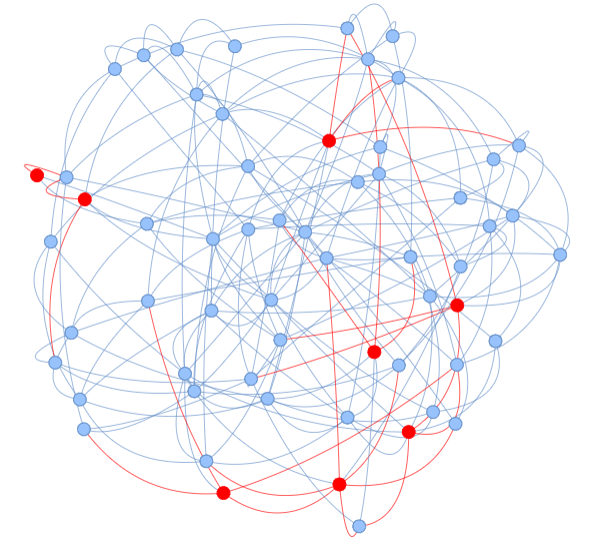
\includegraphics[scale=0.4]{images/Network for spread right wing extremists.png}
    \hspace{1cm}
    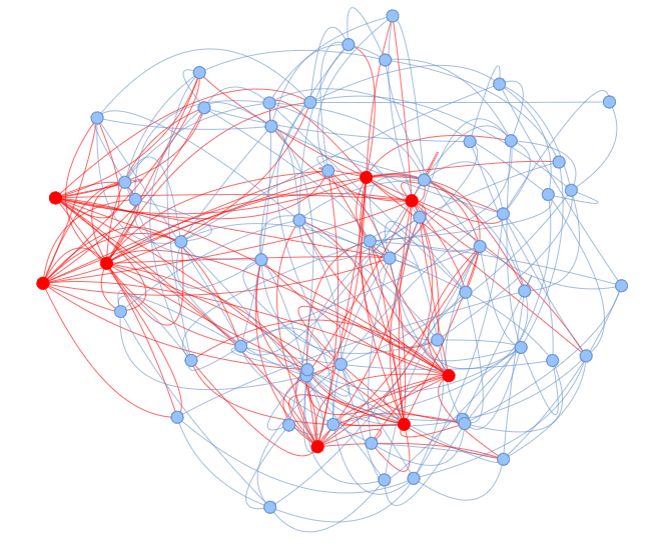
\includegraphics[scale=0.4]{images/Network for political party simulation.png}
    \caption{Normal people shown in blue, and right-wing extremists shown in red. (Left) Network 1, where right-wing extremists are spread across the population with no defined strong connections to each other. (Right) Network 2, where right-wing extremists form small groups and actively seek to push the ideology of the population towards the right. }
\end{figure}

Both networks were simulated for 250 time steps. The evolution of the beliefs of the right-wing extremist group was evaluated for both networks. The figure below shows these results.

\begin{figure}[h]
    \centering
    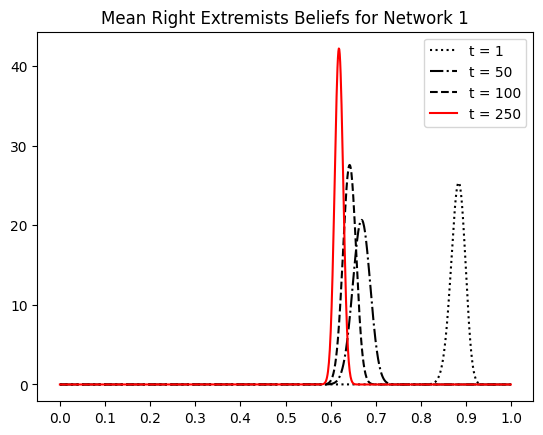
\includegraphics[scale=0.5]{images/Mean right extremist beliefs from spread right extremists.png}
    \hspace{1cm}
    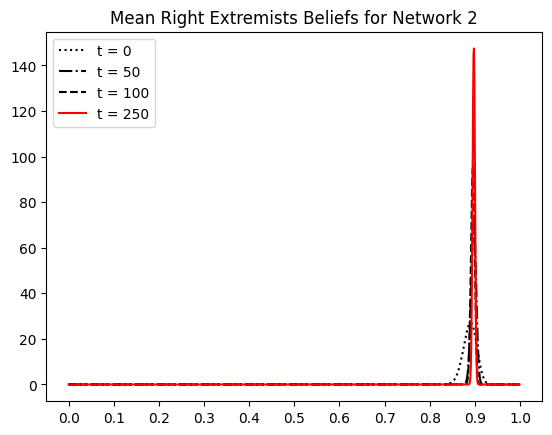
\includegraphics[scale=0.5]{images/Mean right extremist beliefs from political party simulation.png}
    \caption{(Left) Evolution of the mean beliefs of right-wing extremists from Network 1, where right-wing extremists are spread across the population with no defined strong connections to each other. (Right) Evolution of the mean beliefs of right-wing extremists from Network 2, where right-wing extremists form small groups and actively seek to push the ideology of the population towards the right. }
\end{figure}

The results above show the effect of the formation of echo chambers. If extremists are just spread across the population and don't form groups, they can de-radicalize with time. However, if they associate with each other, their radical beliefs remain stable through time, unchanged by the influence of those outside of their community. Our model is capable of representing this complex social dynamic, so this is definitely a good result.

We can also evaluate the evolution of the  beliefs of those who are not part of the right-wing extremist group. This results are shown below.

\begin{figure}[h]
    \centering
    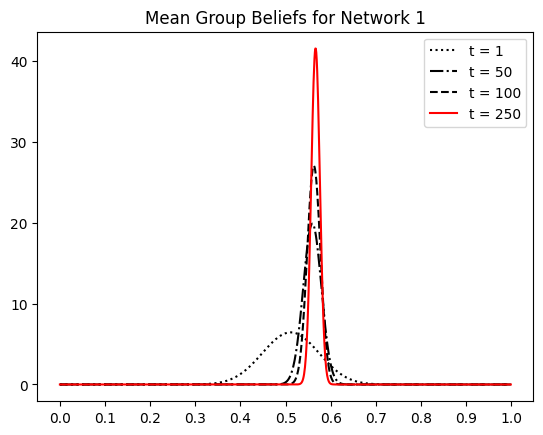
\includegraphics[scale=0.5]{images/Mean group beliefs from spread right extremists.png}
    \hspace{1cm}
    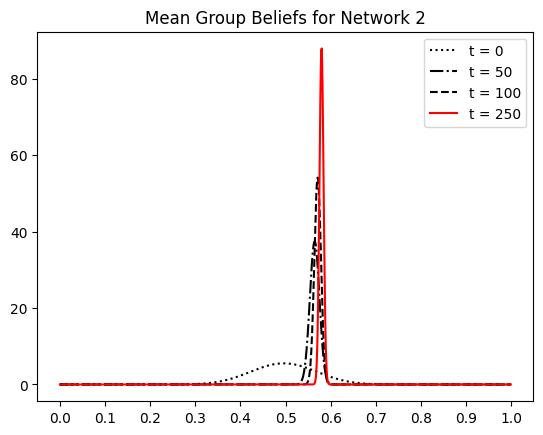
\includegraphics[scale=0.5]{images/Mean group beliefs from political party simulation.png}
    \caption{(Left) Evolution of the mean beliefs of non-extremists from Network 1, where right-wing extremists are spread across the population with no defined strong connections to each other. (Right) Evolution of the mean beliefs of non-extremists from Network 2, where right-wing extremists form small groups and actively seek to push the ideology of the population towards the right. }
\end{figure}

Our results show that there was no significant difference in the change of the beliefs of the non-extremist groups between Network 1 and Network 1. This means that under the defined conditions of the simulation, right-wing extremism did not end up being the dominant ideology. 

This makes sense, because even if there are small groups of extremists whose ideology remains unchanged, and even if these groups try to influence a lot of people, as long as non-extremists have connections between each other, they will resist radicalization. A simulation where extremism ends up being the dominant ideology would probably require more isolated non-extremists and a larger starting number of extremists.

\section{Conclusions}

Condensing the entire complexity of political beliefs into a simple beta distribution is a vast oversimplification. However, as seen above, it is enough to generate complex social dynamics that emerge from the interaction between individuals. We consider our approach to be a successful one, because it allowed us to replicate real-world phenomena like individuals who connect two social groups, the effect of news media sources in the population, and the effect of the formation of radical echo chambers.

Given more time, it would be interesting to experiment with a similar model where beliefs are represented by multivariate distributions. In reality, the left-right division is only a small part of the entire political spectrum, because it only refers to the economic stances of individuals. More complete models of political ideology include a progressive-conservative axis, a libertarian-authoritarian axis, and several others. 

Another interesting future step for the model would be to make trust a function instead of a fixed parameter. This would allow us to make the behaviors of individuals more realistic. For example, we could include cognitive biases like confirmation bias, which states that individuals give more weight to evidence that aligns with what they already belief. In our model, that would look like individuals trusting more those who already align with their ideologies. This would likely allow us to represent even more complicated and interesting social dynamics.

\section{Member Contributions}

\subsection{Design and Implementation}

Marcelo designed and implemented the models for individual conversations and how beliefs are updated. 

Daniel designed and implemented the Person (nodes) and Relationship (edges) classes which facilitate the creation of social networks.  

Both team members designed and implemented several of the networks used for examples throughout this report.

\subsection{Report Writing}

The Explanation and Motivation section was written primarily by M arcelo. The Approach section was written primarily by Daniel. The Results section and Conclusion section were each written collaboratively.

\bibliographystyle{ieeetr}
\bibliography{refs}

\end{document}
